\section{Funktionen}
Eine Funktion $f$ ordnet jedem Element $x$ aus einem Definitionsbereich $D$ genau einen Wert $f(x)$ zu.

\subsection{Grundbegriffe}
\begin{itemize}
\item \textbf{Definitionsbereich $D$}: alle $x$, für die $f(x)$ definiert ist.
\item \textbf{Wertebereich $W$}: alle Werte $f(x)$, die tatsächlich auftreten.
\item \textbf{Graph}: Menge aller Punkte $(x,f(x))$ im Koordinatensystem.
\end{itemize}

\subsection{Wichtige Eigenschaften}
\begin{itemize}
\item \textbf{Stetigkeit}: Eine Funktion ist stetig, wenn man sie zeichnen kann, ohne den Stift abzusetzen.*
\item \textbf{Monotonie}: Eine Funktion ist monoton steigend, wenn $f(x_1) \leq f(x_2)$ für alle $x_1 < x_2$ gilt. Analog für monoton fallend. Bei \emph{strenger} Monotonie gilt $f(x_1) < f(x_2)$.
\item \textbf{Symmetrie}: Eine Funktion ist \emph{gerade}, wenn $f(-x) = f(x)$ gilt, und \emph{ungerade}, wenn $f(-x) = -f(x)$ gilt.\\
    % Graphen einer geraden Funktion
    \pgfplotsset{ticks=none}
    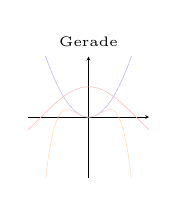
\begin{tikzpicture}[scale=.45]
        \begin{axis}[axis lines=middle, xmin=-2, xmax=2, ymin=-2, ymax=2, width=5cm, height=5cm, yticklabel={\empty}, xticklabel={\empty}]
            \addplot[domain=-2:2, samples=100, blue!30] {x^2};
            \addplot[domain=-2:2, samples=100, orange!30] {-x^4 + x^2};
            \addplot[domain=-2:2, samples=100, red!30] {cos(deg(x))};
        \end{axis}
      \node[anchor=south] at (current bounding box.north) {\tiny{Gerade}};
    \end{tikzpicture}
    \pgfplotsset{ticks=none}
    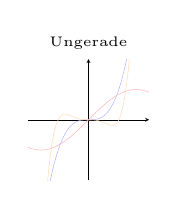
\begin{tikzpicture}[scale=.45]
        \begin{axis}[axis lines=middle, xmin=-2, xmax=2, ymin=-2, ymax=2, width=5cm, height=5cm, yticklabel={\empty}, xticklabel={\empty}]
            \addplot[domain=-2:2, samples=100, blue!30] {x^3};
            \addplot[domain=-2:2, samples=100, orange!30] {x^5 - x^3};
            \addplot[domain=-2:2, samples=100, red!30] {sin(deg(x))};
        \end{axis}
      \node[anchor=south] at (current bounding box.north) {\tiny{Ungerade}};
    \end{tikzpicture}
\end{itemize}

\subsection{Nullstellen}
Eine Nullstelle einer Funktion $f$ ist ein Wert $x_0$ mit $f(x_0) = 0$.

\subsection{Operationen}
Seien $f$ und $g$ zwei Funktionen von einer beliebigen Menge $D$ in $\mathbb{R}$. Dann sind folgende Operationen definiert:
\begin{itemize}
\item \textbf{Addition}: $(f+g)(x) = f(x) + g(x)$
\item \textbf{Subtraktion}: $(f-g)(x) = f(x) - g(x)$
\item \textbf{Multiplikation}: $(f\cdot g)(x) = f(x) \cdot g(x)$
\item \textbf{Division}: $\left(\frac{f}{g}\right)(x) = \frac{f(x)}{g(x)}$, \: $g(x) \neq 0$
\end{itemize}

\subsubsection{Komposition}
Die Komposition von Funktionen $f:A \rightarrow B_f$ und $g:B_g \rightarrow C$ ist definiert als 
\[(g \circ f)(x) = g(f(x)).\]
\emph{Voraussetzung: $B_f \subseteq B_g$}

\subsection{Umkehrfunktionen}
$f$ besitzt eine Umkehrfunktion $f^{-1}$ genau dann, wenn $f$ \textbf{injektiv} ist.  
\[(f^{-1})'(y)=\frac{1}{f'(x)}\quad\text{mit }y=f(x).\]
\textit{Erklärung: Eine Umkehrfunktion ``dreht'' die Zuordnung um; ihre Steigung ist der Kehrwert der ursprünglichen.} \\
